\chapter{Additional Figures}
\label{chap:figures}

\begin{figure}[h]
	\centering
	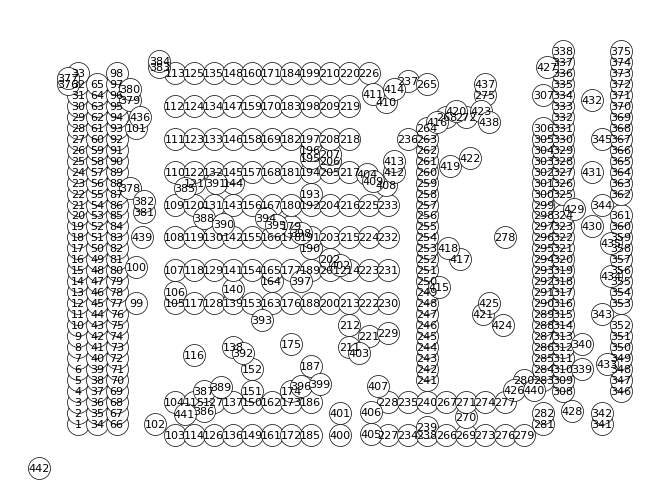
\includegraphics[width=0.6\textwidth]{pcb442.png}
	\caption{Visualization of the \gls{tsp} instance \textit{pcb442}.}
	\label{fig:pcb442}
\end{figure}
\begin{figure}[h]
	\centering
	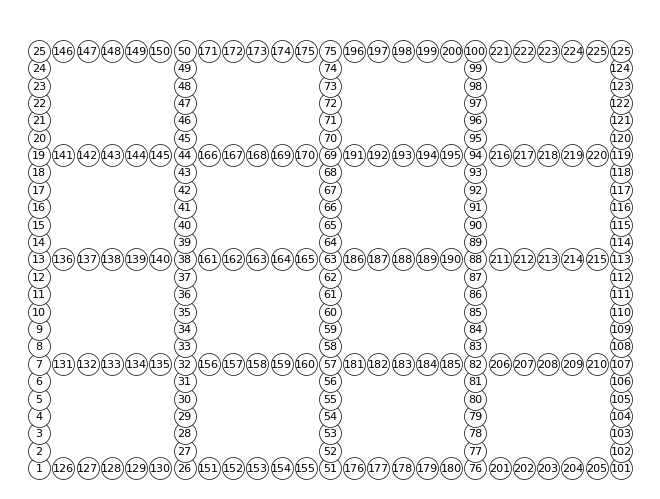
\includegraphics[width=0.6\textwidth]{ts225.png}
	\caption{Visualization of the \gls{tsp} instance \textit{ts225}.}
	\label{fig:ts225}
\end{figure}

\begin{figure}[h]
	\centering
	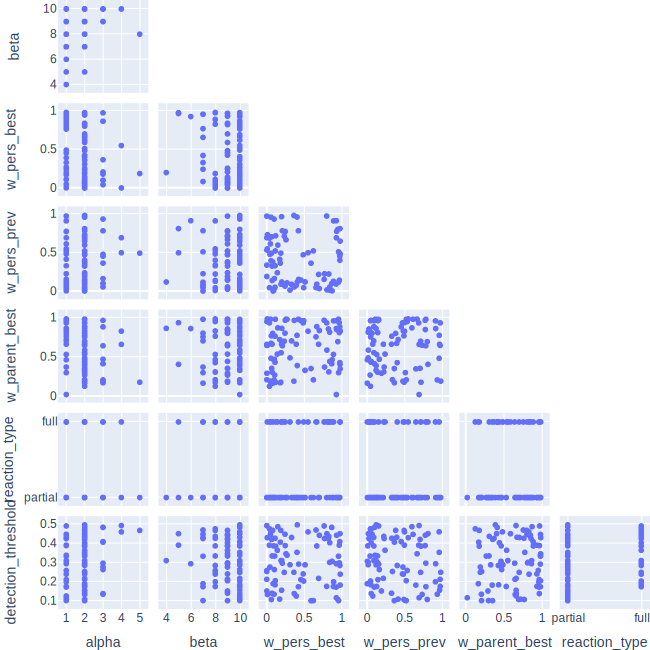
\includegraphics[width=\textwidth]{results/part2/param_scatter_matrix_None_with_H.svg}
	\caption[Scatter matrix plot of all \gls{hsppbo} parameters]{Scatter matrix plot of all \gls{hsppbo} parameters (except $H$) over all 90 optimizer runs with reaction type.}
	\label{fig:parameter_scatter_matrix_added}
\end{figure}
\begin{figure}[h]
	\centering
	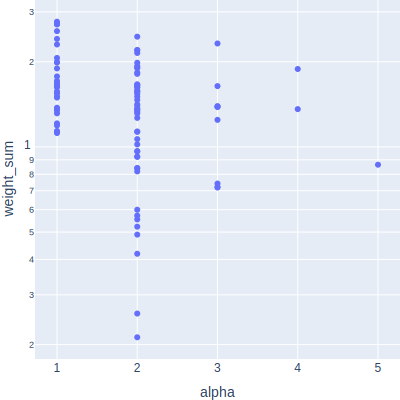
\includegraphics[width=0.6\textwidth]{results/part2/alpha_weight_semilog_plot.svg}
	\caption[Scatter plot of all $\alpha$-values over the sum of the three weights]{Scatter plot of all $\alpha$-values over the sum of the three weights on a logarithmic scale over all 90 optimizer runs.}
	\label{fig:alpha_weight_semilog_plot}
\end{figure}

\begin{figure}[h!]
	\centering
	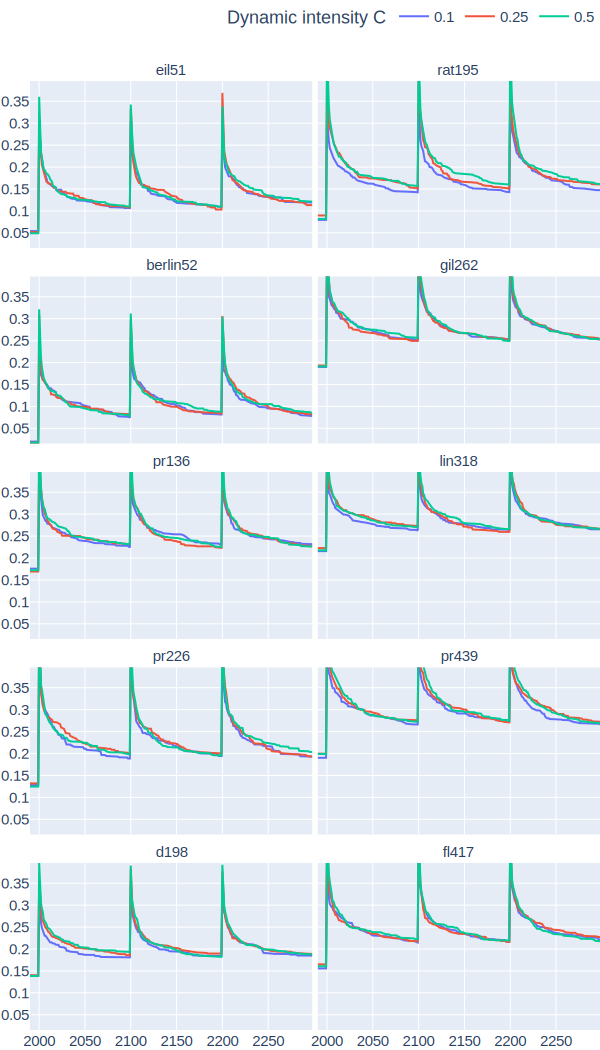
\includegraphics[width=0.725\textwidth]{results/part3/run_plot_cmp_dynamic_aggr_problem_y_best_solution_1_to_30_Reference.svg}
	\caption[Line plots showing the relative solution quality $RPD$ over dynamic iterations for all dynamic intensities $C$ and all \gls{tsp} instances for the \gls{hpo} experiments.]{Line plots showing the relative solution quality $RPD$ over the first 300 dynamic iterations (starting just before iteration 2000) for all three dynamic intensities $C$ and all ten \gls{tsp} instances for the reference experiments. The smaller instances are in the left column and the larger instances are in the right column. Each row corresponds to the predefined structural groups (see \cref{fig:cluster-groups}).}
	\label{fig:run_plot_cmp_dynamic_aggr_problem_ref}
\end{figure}

\begin{figure}[h]
	\centering
	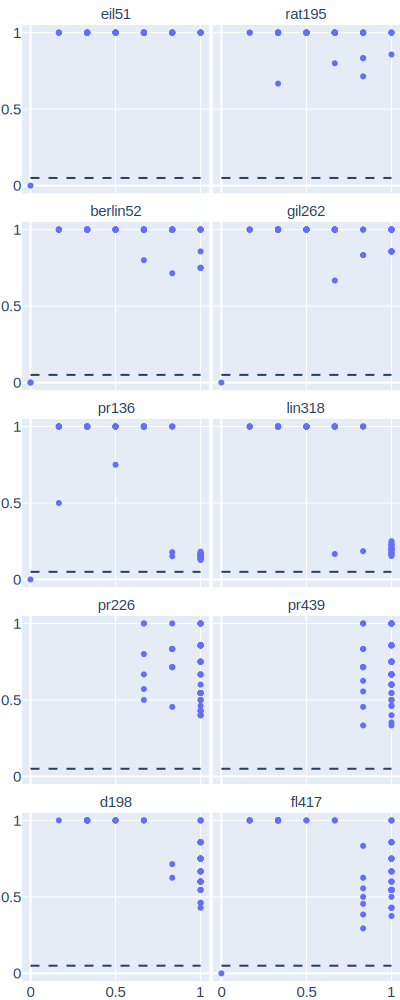
\includegraphics[width=0.5\textwidth]{results/part3/pr_curve_cmp_problem_grouped_False_HPO.svg}
	\caption[Precision-Recall scatter plots separated by \gls{tsp} instance for the \gls{hpo} parameter sets]{Precision-Recall scatter plots showing the values for recall on the x-axis and precision on the y-axis separated for each of the 10 \gls{tsp} instances (name atop the plots) for the \gls{hpo} parameter sets. The smaller instances are in the left column and the larger instances are in the right column. Each row corresponds to the predefined structural groups (see \cref{fig:cluster-groups}).}
	\label{fig:pr_curve_cmp_problem_HPO}
\end{figure}
